\section*{Analiza porównawcza spójności wyjaśnień}
W tej sekcji przeprowadzimy analizę spójności wyjaśnień generowanych przez różne metody XAI: LIME, SHAP i GradCAM.
Naszym celem jest ocena, jak bardzo wyjaśnienia nakładają się na siebie oraz jak różne techniki identyfikują istotne cechy obrazu.

W celu oceny spójności wyjaśnień, każda z metod XAI została użyta do wygenerowania wyjjaśnień dla tego samego zestawu obrazów.
Wyniki były przedstwaione za pomocą metryki IoU, która mierzy stopień pokrycia się regionów uznawanych za istotne przez różne metody.

\begin{figure}
	\centering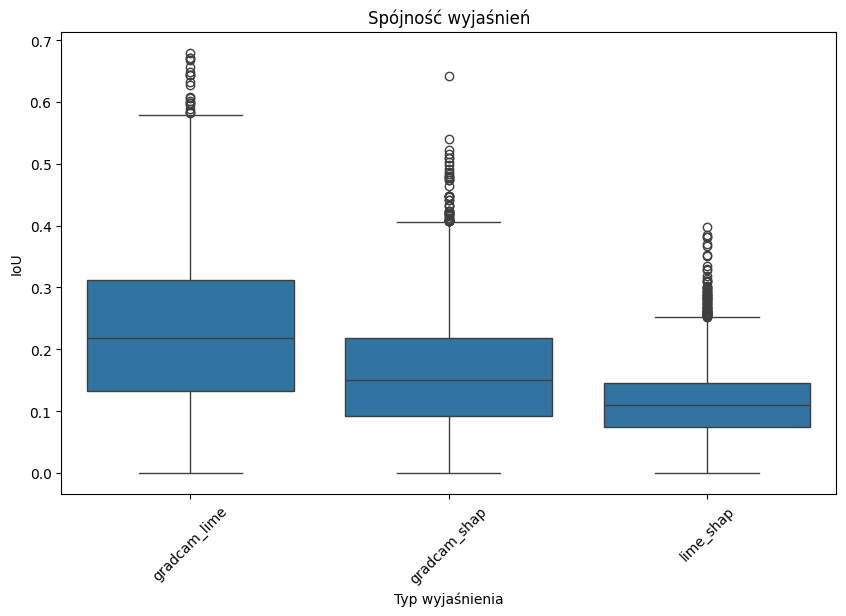
\includegraphics[width=.6\textwidth]{img/base_coherence}
	\caption{Spójność wyjaśnień}  \label{rys:base_coherence}
\end{figure}

Na rys \ref{rys:base_coherence} został przedsawiony wykres pudełkowy wartości IoU.
Średnia wartość IoU dla GradCAM i LIME jest równa 0.229, dla GradCAM i SHAP 0.162 oraz dla LIME i SHAP 0.114.
Największą spójność posiadają wyjaśnienia wygenerowane przez GradCAMa oraz LIME.
Najmniejszą natomiast mają wyjaśnienia wygenerowane przez LIME oraz SHAPa.

Aby lepiej zrozumieć, spójność wyjaśnień, możemy przeprowadzić te same badania dzieląc wyniki na kategorie obrazów.

\begin{figure}
	\centering
	\begin{minipage}[b]{0.3\textwidth}
		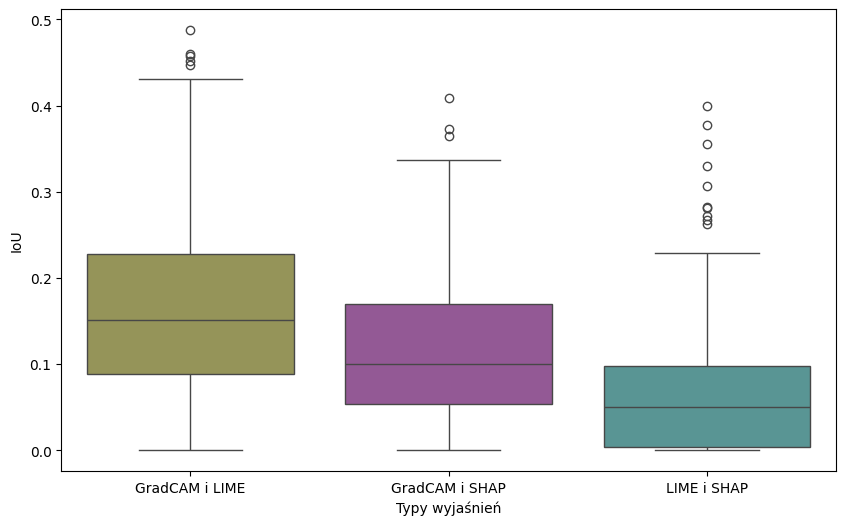
\includegraphics[width=.9\textwidth]{img/base_coherence_dog}
		\caption{Spójność wyjaśnień dla kategorii Dog}  \label{}
	\end{minipage}
	\begin{minipage}[b]{0.3\textwidth}
		\centering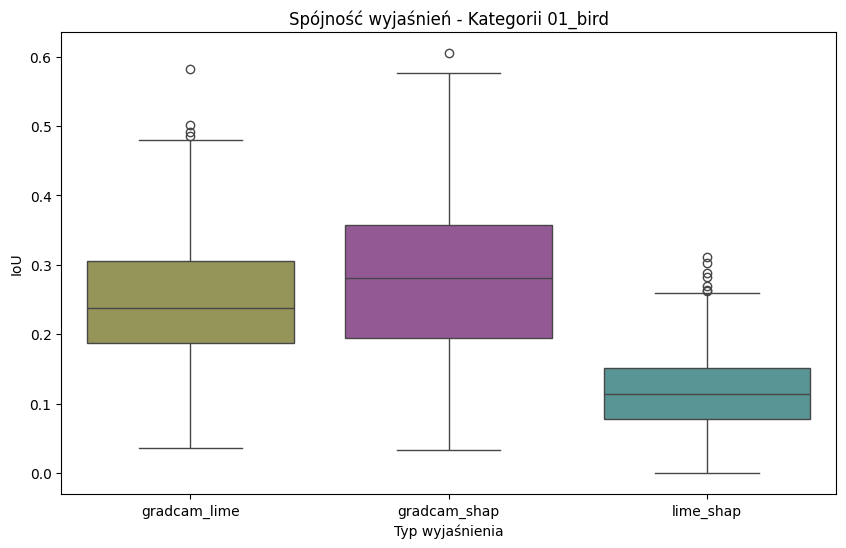
\includegraphics[width=.9\textwidth]{img/base_coherence_bird}
		\caption{Spójność wyjaśnień dla kategorii Bird}  \label{}
	\end{minipage}
	\begin{minipage}[b]{0.3\textwidth}
		\centering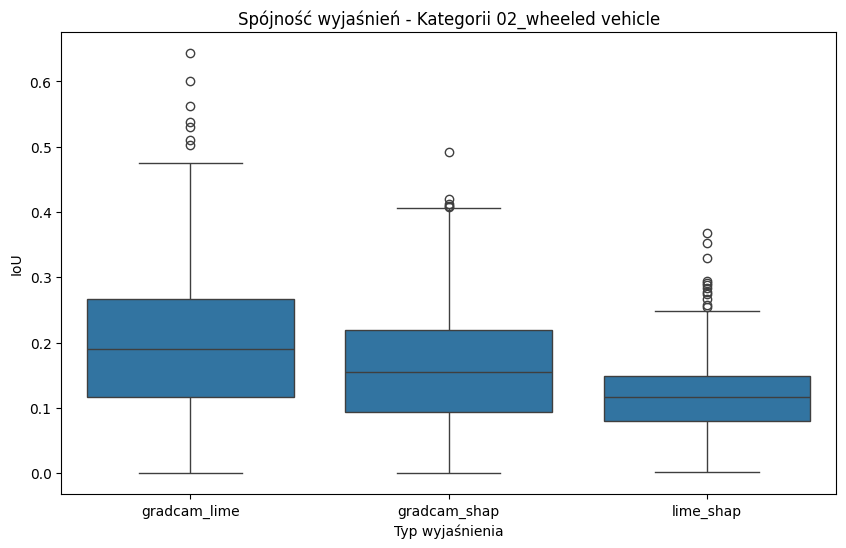
\includegraphics[width=.9\textwidth]{img/base_coherence_vehicle}
		\caption{Spójność wyjaśnień dla kategorii Vehicle}  \label{}
	\end{minipage}
\end{figure}
\begin{figure}
	\centering
	\begin{minipage}[b]{0.3\textwidth}
		\centering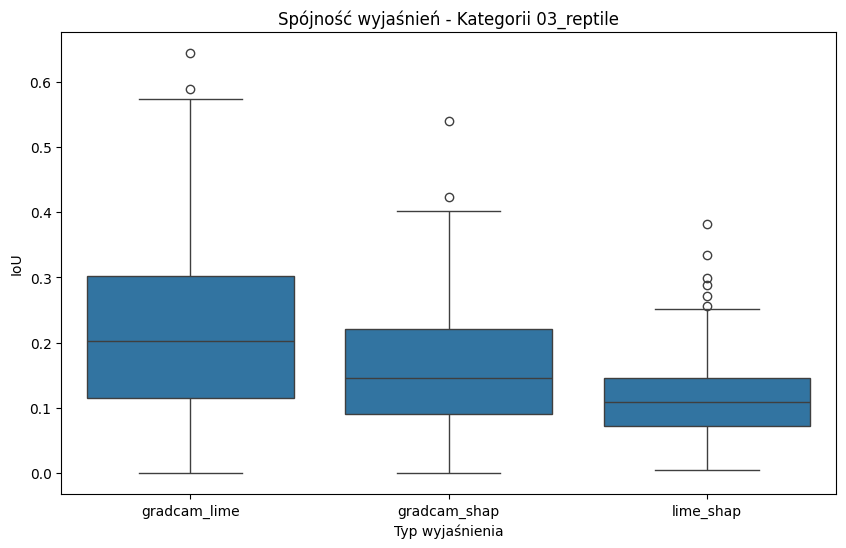
\includegraphics[width=.9\textwidth]{img/base_coherence_reptile}
		\caption{Spójność wyjaśnień dla kategorii Reptile}  \label{}
	\end{minipage}
	\begin{minipage}[b]{0.3\textwidth}
		\centering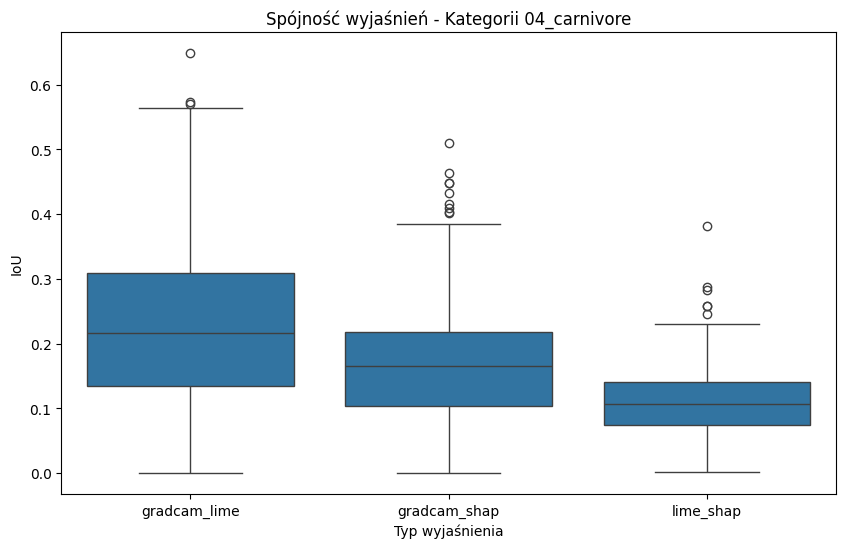
\includegraphics[width=.9\textwidth]{img/base_coherence_carnivore}
		\caption{Spójność wyjaśnień dla kategorii Carnivore}  \label{}
	\end{minipage}
	\begin{minipage}[b]{0.3\textwidth}
		\centering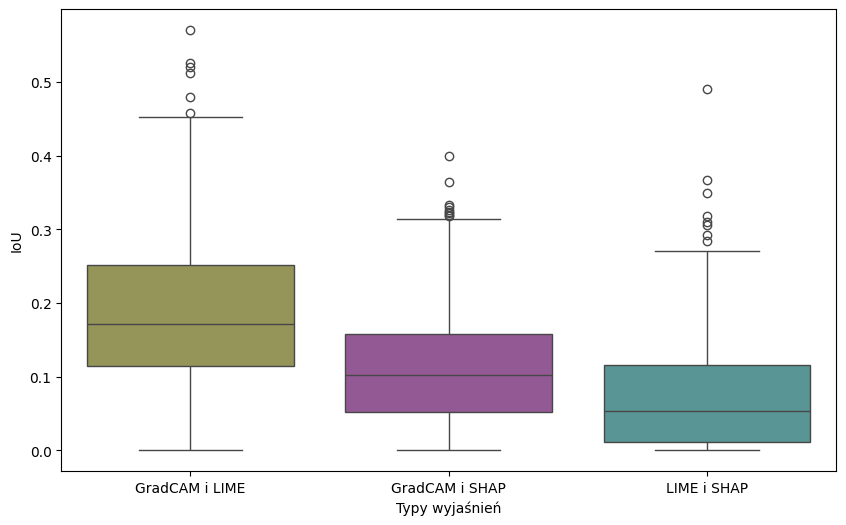
\includegraphics[width=.9\textwidth]{img/base_coherence_insect}
		\caption{Spójność wyjaśnień dla kategorii Insect}  \label{}
	\end{minipage}
\end{figure}
\begin{figure}
	\centering
	\begin{minipage}[b]{0.3\textwidth}
		\centering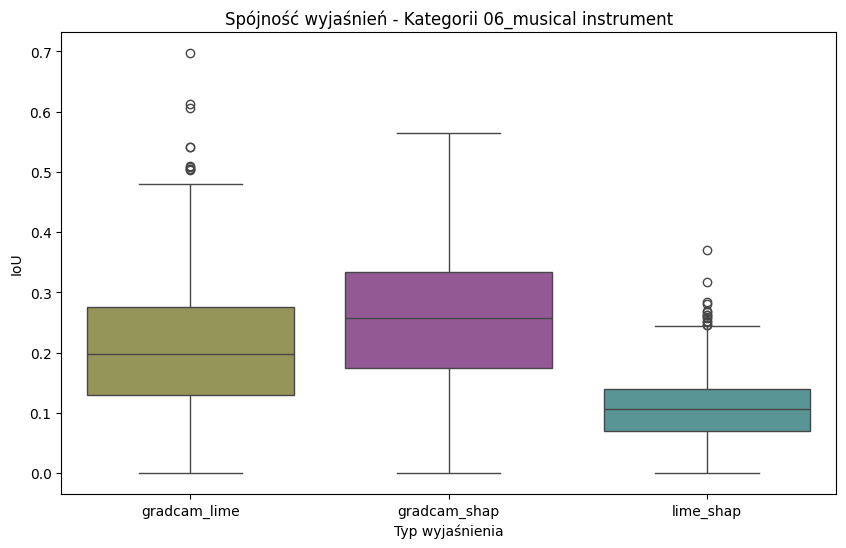
\includegraphics[width=.9\textwidth]{img/base_coherence_music}
		\caption{Spójność wyjaśnień dla kategorii Instrument}  \label{}
	\end{minipage}
	\begin{minipage}[b]{0.3\textwidth}
		\centering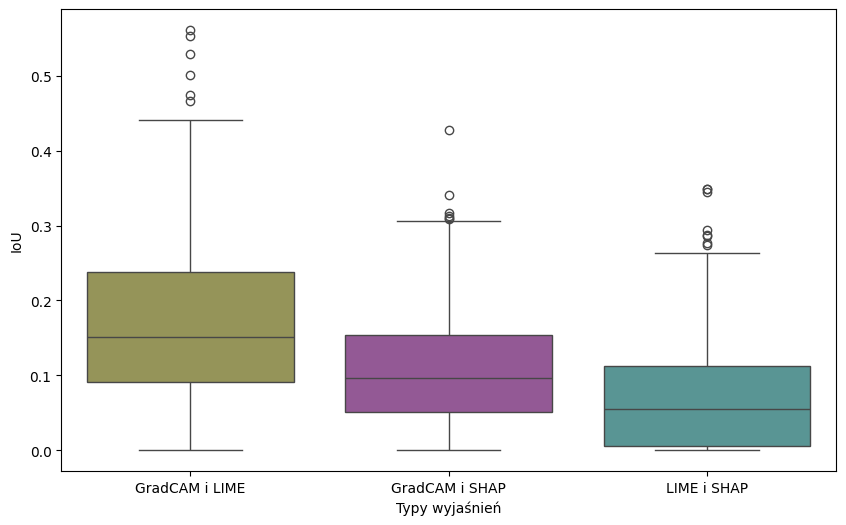
\includegraphics[width=.9\textwidth]{img/base_coherence_primate}
		\caption{Spójność wyjaśnień dla kategorii Primate}  \label{}
	\end{minipage}
	\begin{minipage}[b]{0.3\textwidth}
		\centering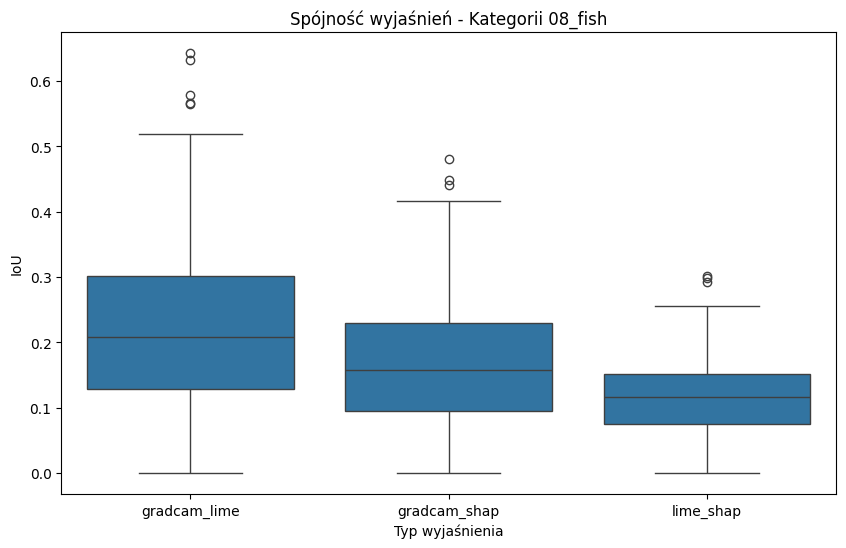
\includegraphics[width=.9\textwidth]{img/base_coherence_fish}
		\caption{Spójność wyjaśnień dla kategorii Fish}  \label{}
	\end{minipage}
\end{figure}

Dla wszystkich kategorii wygląda to podobnie, GradCAM i LIME posiadają najwyższą spójność, a LIME i SHAP najniższą.
